%\documentclass[a4paper,bibtotoc]{scrartcl}
\documentclass[a4paper,bibtotoc]{scrartcl}

\usepackage[english]{babel} %English 
%\usepackage[T1]{fontenc}
\usepackage[utf8]{inputenc} %utf8 encoding
\usepackage[colorlinks]%, %Anstatt Boxen um Links, diese einfärben
        	{hyperref}		%Anklickbare Links
\usepackage{graphicx}
\usepackage{algorithmic}

\interfootnotelinepenalty=10000 % this prevents footnotes from being split across multiple pages
%\usepackage{
%	amsmath,                 % improves quality of formulas
%   amssymb,                 % mathematical symbols
%   amsfonts,                % mathematical fonts
%   amsthm,                  % macros for theorems, lemmas, etc.
%   graphicx,                % needed to include graphics and images
%}

\newcommand{\totype}{\(\to\;\)}

\title{KeyChain Extension and Integration\\
	Final Report}
\subtitle{Practical Lab on Smartphone Security}
\author{Kjell Braden, Marvin Dickhaus, Cassius Puodzius}
\date{Winter term 2012/2013\\\today}


%%% START OF DOCUMENT %%%%%%%%%%%%%%%%%%%%%%%%%%%%%%%%%%%%%%%%%%%%%%%%%%%%%%%%

\begin{document}

\maketitle

\begin{abstract}
	The goal of this project is to extend the built-in key storage of Android 4.2 to support functionality such as signing and decrypting without revealing the needed key to any app.\\
	The second goal is the integration of system apps to demonstrate the functionality. This group implemented symmetrically encrypted SMS for that purpose.
\end{abstract}

\tableofcontents
% TODO shorten abstract or put TOC on own page, currently it gets split
%\pagebreak[4]


\section{Introduction}
	Since Android API Level\footnote{\url{http://developer.android.com/guide/topics/manifest/uses-sdk-element.html\#ApiLevels}} 14 (4.0 Ice Cream Sandwich) the \texttt{KeyChain}\footnote{\url{http://developer.android.com/reference/android/security/KeyChain.html}} class exists in Android. The \texttt{KeyChain} class allows storage of asymmetric keys in a secure credential storage.

	In default implementation an authorized app is always able to retrieve the private key. Our goal was to extend the given functionality further with a crypto oracle, as well as support for different key types, both symmetric and asymmetric. With that functionality, apps should call the API with the data they want en-/decrypted or signed/verified. In the process of en-/decryption and signing the API returns the respective byte data. In verification the API returns a boolean indicating whether it had success or failure.
	
	Besides the new API, we wanted to alter at least one system app to comply with our enhanced KeyChain. After suggestions from Sven Bugiel (our supervisor) we decided to implement a symmetric encryption with the SMS app instead of the E-Mail app (More on that in section \ref{sec-sms-app}).

\section{Initial Situation}
	At the starting point, we were confronted with a quite unfinished, not wholly tested API. Furthermore the KeyChain API lacks in documentation. So we had to figure out how it would be possible to implement our functionality. The following listing gives an overview of the need-to-know classes for this project:
	
	\begin{description}
		\item[KeyChain] is the Android API for importing PKCS\#12 containers (private keys, public key certificates and CA certificates) and providing grant-based access of the keys to apps. The PKCS\#12 format requires the container to be encrypted.
			\begin{itemize}
				\item When an import is requested the API creates an Intent, which is handled in the system app \path{com.android.certinstaller} (source at \path{packages/apps/CertInstaller/CertInstaller.java} et al.). CertInstaller spawns a dialog and handles the container decryption process as well as stores the keys in the \texttt{keystore} daemon (see below).
				\item Keys are identified by aliases, which are chosen by the user when the CertInstaller is invoked with an import request.
				\item Private as well as public keys (in the form of certificates) can be requested:
				\begin{itemize}
					\item If access to a private key was granted to the requesting app, it can be retrieved using \texttt{getPrivateKey()}.
					\item Public keys can be retrieved through \texttt{getCertificateChain()}
				\end{itemize}
			\item \texttt{KeyChain} also contains \texttt{AndroidKeyPairGenerator} since Android 4.2, which generates and stores key pairs in \texttt{key\-store} automatically.
			\end{itemize}

		\item[KeyChain app] is a system application implementing most parts of the \texttt{KeyChain} API. It grants key access to apps and retrieves keys from the secure native \texttt{keystore} daemon (see below).

		\item[keystore] is the native daemon (written in C++) that holds encrypted key information.
			\begin{itemize}
				\item The storage is encrypted with a master key which is derived from the unlock passphrase, PIN or pattern of the device\footnote{In order to import and use certificates that are not in the trusted certificates from the Android base (known as user certificates), respectively use the \texttt{keystore}, a PIN, passphrase or pattern has to be created, that will unlock the device.}.
				\item Unlocks on the \emph{first successful unlock attempt} of the device, won't lock again \emph{until the phone is powered off}. This means the keystore is protected for example from rooting, but not from live-debugging. (It is possible for apps to lock it manually, though.)
				\item The service supports two storage types:
				\begin{description}
					\item[key] is a RSA key pair. Once stored the private key cannot be exported again, more on this later.
					\item[blob] can be arbitrary data.
				\end{description}
				\item \texttt{keystore} provides an OpenSSL engine called \texttt{keystore}, which should be able to retrieve PrivateKey objects from the daemon directly in Java code.
			\end{itemize}
		\item [CertInstaller] The \texttt{CertInstaller} is a system app that lets a user import and install key pairs and certificates from PKCS\#12 container format files. %TODO: Expand!
	\end{description}

	\subsection*{Detour: Java Cryptography Architecture (JCA)}
		The JCA is a {\em provider framework} for common cryptography operations such as hashing, sign/verify, encrypt/decrypt and key/certificate generation. Each of these operations have an algorithm- and implementation-independent interface, most of which operates on objects implementing the \path{javax.crypto.SecretKey}, \path{java.security.PublicKey} or \path{java.security.PrivateKey} interfaces, depending on the context.

		This makes it possible for crypto code to be written largely independent on actual implementation e.g. of the keys.

	\section{Requirements}
		To achieve our goal, we need to be able to securely store and generate both symmetric and asymmetric keys, regardless of the key type.

		Apps should be able to do crypto operations with specific keys. In order to access those keys, the user should be required to give his permission. The operations necessary can be distinguished by the key type.
		\begin{itemize}
			\item For private keys, operations include decryption and signing of data.
			\item For public keys it's encryption and verification.
			\item With symmetric keys, apps need to be able to both en-/decrypt, as well as sign and verify, which means generating and checking {\em message authentication codes (MAC)} in this case.
		\end{itemize}

		These operations must not leak any kind of private key parameter or any part of the symmetric key used.

		For convenience, it would be a good idea to create and store key exchange (eg. Diffie-Hellman) parameters as well, and to automatically derive and store the resulting symmetric key on receiving the remote's parameters. %TODO: Explain this further.

	\subsection{Workflow with the existing KeyChain API}
		% don't remove this linebreak, tex seems to have issues wrapping this line correctly.
		In the KeyChain API there are \texttt{AndroidKeyPairGenerator}, \texttt{AndroidKeyStore} \linebreak and \texttt{KeyChain}.

		The \texttt{AndroidKeyPairGenerator} implements JCA's \texttt{KeyPairGenerator} interface and sends a key generation request to the \texttt{keystore} daemon. In this vein, the keys' types are hard coded to {\em 2048 bit RSA}. The \texttt{AndroidKeyStore} implements the \texttt{KeyStore} interface. It retrieves the key references from the daemon, but does no permission checking. If the requesting app has never been granted access to the requested key, the access simply fails. Additionally, it only supports asymmetric keys.

		Key references means that the returned key objects don't carry the cryptographic parameters themselves, but instead they are handles that the OpenSSL JCA provider can use to run the crypto operations on the keys in the \texttt{keystore}, so the Java code (and specifically, the app's code) never sees any crypto parameters at all. The \texttt{KeyChain} allows to retrieve \texttt{PrivateKey} using the \texttt{AndroidKeyStore}, but requests permission to access a key beforehand. The user will see a dialog telling him which app tries to access a key, can choose the one he wants to use and the app gets access to that granted key. 
		
	\subsection{Proposed Implementation Ideas}
		\subsubsection{Reuse KeyChain API}
			Our initial plan was to reuse as much of the KeyChain API as possible. Nevertheless we would need to add support for symmetric keys and other asymmetric key types in both storage and key generation as well as support for key exchange handling.

			This turned out to be harder than we thought, as we would need to rewrite significant amount of C++ code in the \texttt{keystore} daemon for supporting anything else than RSA. Also we would have to rewrite the protocol the \texttt{keystore} uses to communicate with the Java framework.
			
			On top of that, there turns out to be a bug somewhere in Android's OpenSSL engine, which causes {\em dalvik} to {\em segfault} as soon as encryption or decryption is being run with the returned key references.

		\subsubsection{The manual way}
		After various attempts to reuse existing \texttt{KeyChain} code, we got to a working solution by doing everything in our own code and store the keys as blobs in the \texttt{keystore}. This means:
			\begin{enumerate}
				\item Manually generate the key pair, manually store it in the \texttt{keystore} as a PKCS\#8 (not PKCS\#12) encoded blob and the certificate as PEM encoded blob.
				\item For encryption, manually load the certificate from \texttt{keystore}, parse it, feed it to \path{java.security.Cipher}.
				\item For decryption, manually load the private key from \texttt{keystore}, parse it, feed it to \path{java.security.Cipher}.
				\item For symmetric crypto, we simply store the secret key bytes as blobs in \texttt{keystore}.
			\end{enumerate}

\section{Implementing the framework}

	The framework respectively the back end consists of the \texttt{KeyChain} app for all the crypto operations on the one hand and the management of the keys on the other hand.

	\subsection{Key Chain}
		To reduce responsibility of the apps it makes sense to let the system app (\texttt{KeyChain}) handle everything related to key management:
		\begin{enumerate}
			\item Generate keys
			\item Delete keys
			\item Import/Export of key \emph{pairs}\footnote{Users should be able to export their keys for use on other devices.}
			\item Grant key access to apps
		\end{enumerate}
		Our first sketch didn't quite reflect symmetric encryption, so there was some more work in order to refine our API, with the final result being as follows.

		\begin{enumerate}
		\tt
			\item encryptData(keyId, algorithm, padding, plaintext, IV) \totype ciphertext
			\item decryptData(keyId, algorithm, padding, ciphertext, IV) \totype plaintext
			\item sign(keyId, algorithm, plaintext) \totype signature
			\item verify(keyId, algorithm, plaintext, signature) \totype isValid
			\item storePublicCertificate(keyId, certificate) \totype void

			\item generateSymmetricKey(keyId, algorithm, keysize) \totype void
			\item retrieveSymmetricKey(keyId, algorithm) \totype key
			\item importSymmetricKey(keyId, key) \totype void
			\item deleteSymmetricKey(keyId) \totype void
			\item mac(keyId, algorithm, plaintext) \totype mac

			\item generateKeyPair(keyId, algorithm, keysize) \totype publicKey
			\item keyAgreementPhase(keyId, keyAlgorithm, agreementAlgorithm,
				\linebreak % XXX latex seems to have issues with proper line wrapping in tt
				publicKey, isLastPhase) \totype publicKey
		\end{enumerate}

		Keys itself are referenced by an string alias (\emph{keyId}). Every key has exactly one alias assigned in the \texttt{keystore}. This alias must be unique.
	
		The functions \texttt{encrypt} and \texttt{decrypt} are used for symmetric as well as for asymmetric crypto.

		The functions \texttt{sign}, \texttt{verify} and \texttt{storePublicCertificate} are exclusive to asymmetric crypto.
		%TODO: Describe how an app is granted to use a key!

		\texttt{generateKeyPair} and \texttt{keyAgreementPhase} are intended for key agreement protocols like the Diffie-Hellman key exchange. This way, you can create key agreement parameters (which are handled as \texttt{PrivateKey} and \texttt{PublicKey} objects), transmit them to your communication partner. You then feed in the received parameters using \texttt{keyAgreementPhase} which can return another set of parameters if the protocol is not finished yet, or, if the protocol is finished, it will immediately derive the shared secret key and store it under the alias previously used by the key exchange parameters.

		The other functions are just for symmetric crypto operations.

		The API is made available to apps from the framework in the \texttt{android.security} package, but every call
		is actually forwarded using the Binder IPC to the \texttt{KeyChain} app which runs with system permissions and
		is allowed to do any operation on the \texttt{keystore} daemon. The \texttt{KeyChain} app is therefore responsible
		for checking if requesting apps are allowed to access specific keys before obeying to their requests.
	
	\subsection{Key Management App}
		In addition to all the new crypto operations, keys have to be assigned to contacts. This is realized in the new {\em Key Management} system app. After a key was created or imported, it can be assigned to contacts. Each assignment gets a new string identifier (called {\em usage type}) which is arbitrary but application defined. For example a crypto e-mail could get \textit{mail-crypt} as usage type. Now whenever an encrypted e-mail is sent to a contact, the program only has to check if a key with this usage type is present. If not, no key for this usage is defined and so encryption can't happen. This way the user can decide which key to use for which application, and easily replace keys once they are obsolete.
		
		Each usage type has to be unique per contact. It is also possible to assign the same key more than once to a contact, provided that the usage type is different each time. For example, a user could use the same key for e-mail and SMS encryption.

		The key assignments are stored with a MIME type of \texttt{vnd.android.cursor.item/key} in the \texttt{ContactsContract.Data} table of the {\em Android contacts provider\footnote{\url{http://developer.android.com/guide/topics/providers/contacts-provider.html}}}.
		
\section{Integrating the SMS app with our API}
	\label{sec-sms-app}
	
	\subsection{Considerations}
		At first we thought about integrating asymmetric cryptography with the standard e-mail app. Sven Bugiel brought to our attention that extending the default e-mail app would be quite complicated and would bear a huge overhead. Instead he suggested to take on SMS as this would be more feasible. As asymmetric crypto bears a huge overhead for SMS (in terms of message size and therefore cost per SMS) we decided to implement symmetric cryptography with the SMS app instead. %TODO: Is this enough for the part of "Why"? [I think so (Cassius)]
	
		In this scenario, we assumed that the symmetric key would already be exchanged with the other party. So we just had to handle sending and receiving SMS.
	
		The greatest inconvenience with system apps is that one first has to build the image once you developed something. As compiling Android even on powerful systems takes hours, we decided against altering the system app and instead overlaying it. This means:
		\begin{itemize}
			\item For writing encrypted messages, a separate UI is needed.
			\item For receiving encrypted messages, broadcasts need to be captured.
			\item In every case, the unencrypted messages are stored in the communication log with the respective contact.
		\end{itemize}
		This also means, other than when sending encrypted SMS, the user doesn't have to differ from his known behavior.
		
	\subsection{Implementation Details}
		\subsubsection{Sending}
			Since outgoing messages can't be intercepted and modified, there needs to be separate custom activity for composing encrypted messages.  The layout is very simple. It consists of a contact field, a text field and a send button. See figure \ref{fig:compose}.
			\begin{figure}[h]
				\centering
					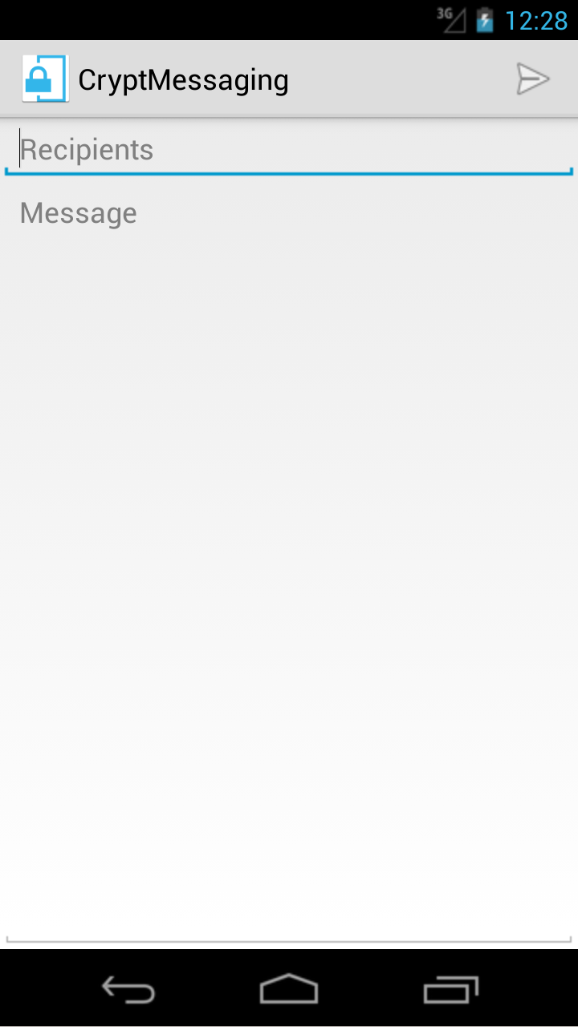
\includegraphics[width=15em]{crypt-compose.png}
				\caption{The layout of encrypted SMS composing.}
				\label{fig:compose}
			\end{figure}

			Contacts are only selectable if they have already a key with the {\em usage type} of \texttt{sms-symmetric} defined. After composing is finished, the user sends the SMS with the send button. The text will then be encrypted with the given symmetric key and encoded in Base64. To identify encrypted SMS when they are received, the @-character will be appended at the beginning and the end.

			Outgoing messages are stored in the (undocumented) SMS content provider \linebreak % check draft and linewrapping before removing
			\texttt{content://sms}, so they can appear in the regular conversation history and receive status updates (for example a delivery notification). Then they are encrypted and sent, in multiple parts, if necessary, using the Android API \texttt{SmsManager}.

		\subsubsection{Receiving}
      For receiving SMS, apps need to intercept the \texttt{SMS\_RECEIVED} broadcast with a high priority, before any other app can handle them. After being processed a notification is shown and the decrypted message will be stored in the SMS content provider as well.
      
      Once the user has assigned a \texttt{sms-symmetric} key to a contact, decrypting SMS works without any interference of the user. Basically, the steps of decrypting are reverse to encrypting. If a broadcast for a new incoming SMS is received, then:

			\begin{algorithmic}
				\STATE {\tt Check if the SMS is encrypted after all parts were received\footnote{@-char at the beginning and end}}
				\STATE {\tt Check if the sender has a key assigned}
				\IF{No key is assigned to the sender}
					\STATE {\tt Abort broadcast}
				\ELSE
					\STATE {\tt Decrypt SMS}
					\STATE {\tt Store decrypted SMS in the conversation log}
				\ENDIF
			\end{algorithmic}

\section{Key Exchange Scenarios}
	Since apps running as the system user (ie. with user id 1000) are not generally allowed to write to the sd card,
	exporting keys from the key management app is implemented by using a \texttt{ACTION\_SEND} intent with a MIME type
	of \texttt{*/*}. This way, the operating system automatically offers to send the key file for example as an attachment
	via e-mail or via bluetooth. It should be easy to extend this functionality to Near Field Communication.

	The receiving party receives the key file and can import it in their key management app. Before importing though,
	this should display key fingerprints (or any other hash visualization scheme\footnote{as discussed in \cite{perrig99}})
	to allow verification between both parties.
	
\section{Responsibilities}
	%Who did what?
	%Reports - All of us
	%Framework - Kjell, ([Cassius?] I gave only the DH tip, the rest is very much Kjell. Right?)
	%Crypt-SMS-App - All of us with Kjell doing the most?
	
\section{Further development}
	%TODO: What could come next?
	As this project was intended as a proof-of-concept, there are quite a few angles, that leave room for improvement. Some ideas of further development are:
	\begin{enumerate}
		\item When symmetric cryptography is used, MACs have to be compared in user code. The KeyChain could provide a \texttt{verifyMac} method instead.
		\item Provide import and export of keys to QR-Code.
		\item Currently when keys are exchanged between parties, the keys are exposed to non system apps. Instead, NFC could be used to exchange keys directly between two \texttt{keystore} instances and therefore never be exposed to the outside world.
		\item The encrypted SMS app is missing some basic functionalities. Some enhancements that come into mind:
		\begin{enumerate}
			\item Warn the user, if the encrypted SMS is longer than 160 characters, because it cost more money to send them.
			\item Implement a character counter, that encrypts the text on-the-fly and displays used characters of the encrypted SMS.
		\end{enumerate}
		\item A further security consideration would be to store the SMS encrypted on the phone. Of course there are several possible ways to do so.
		\begin{enumerate}
			\item Encrypt SMS with the master key derived from the pin/pattern that locks the phone. This would be the way, the keystore is encrypted, too.
			\item Encrypt with a application specific pin.
		\end{enumerate}
	\end{enumerate}
	%Store encrypted on phone and decrypt with password.

\begin{thebibliography}{9}
	\bibitem{perrig99}
		Adrian Perrig and Dawn Song,
		{\em Hash Visualization: a New Technique to improve Real-World Security}.
		1999.
\end{thebibliography}
\end{document}

